% Метод перестроения поверхности с помощью общей огибающей семейства сфер.
\subsection{Метод окрестностей перестроения расчетной сетки \\ в пространстве}

В этом разделе рассмотрим метод перестроения поверхностной сетки, в котором узлы в процессе перестроения смещаются на границу окрестности одной из инцидентных ячеек.
Этот метод перестроения будем называеть методом окрестностей перестроения поврехности\label{term:method_remesh_okr}.

Рассмотрим геометрическую задачу определения новых положений узлов расчетной сетки, если для каждого узла $N$ известна скорость образования ледяного покрова $v(N)$, измеряемая в метрах в секунду \cite{Rybakov2023GeoRemesh}.
Будем считать, что нарастание льда в любой точке роста льда выполняется одновременно во всех направлениях аналогично принципу Гюйгенса-Френеля распространения волн.
Таким образом, фронт распространения льда от произвольной точки $P$ через промежуток времени $\Delta t$ будет иметь форму сферы $Sphere(P, v(P)\Delta t)$.
Далее будем считать, что мы выполняем расчет новых положений узлов через некоторый фиксированный момент времени $\Delta t$, то есть для каждого узла $N$ известен радиус продвижения фронта ледообразования $R(N) = v(N) \Delta t$.
Так как при выполнении численных расчетов фронт продвижения льда у нас представлен неструктурированной поверхностной расчетной сеткой, ячейки которой имеют форму треугольников, а радиусы продвижения фронта льда заданы только в узлах сетки, необходимо определить радиусы продвижения фронта льда для каждой точки внутри ячейки.

\begin{figure}[ht]
\centering
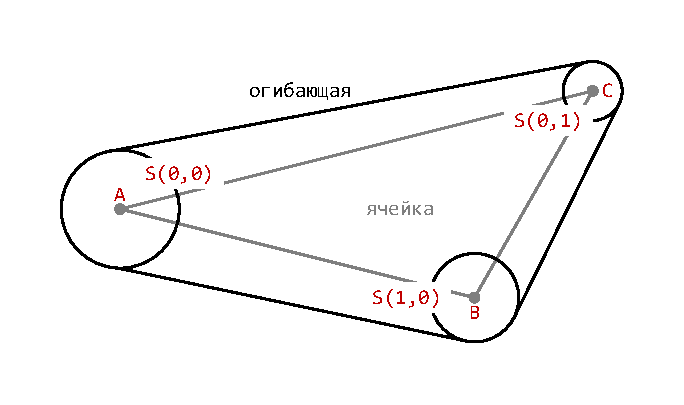
\includegraphics[width=0.6\textwidth]{./pics/text_1_remesh_common_envelope/triangle.pdf}
\singlespacing
\captionstyle{center}\caption{Окрестность ячейки расчетной сетки.}
\label{fig:text_1_remesh_common_envelope_1}
\end{figure}

Рассмотрим некоторую ячейку расчетной сетки, представляющую собой треугольник $Tri(A, B, C)$.
Определим для каждой точки $P(\beta,\gamma)$ внутри треугольника радиус продвижения фронта льда как
\begin{equation}
	R(P(\beta,\gamma)) = R(\beta,\gamma) = R(A) + \beta(R(B) - R(A)) + \gamma(R(C) - R(A))
\end{equation}

и фронт продвижения льда от точки $P(\beta,\gamma)$ представляет собой сферу $Sphere(\beta,\gamma) = Sphere(P(\beta,\gamma),R(\beta,\gamma))$.
Областью продвижения льда для всей ячейки расчетной сетки является окрестность этой ячейки $O_R(ABC)$ (см. рис.~\ref{fig:text_1_remesh_common_envelope_1}).

При изменении положения узлов расчетной ячейки (точки $A$, $B$, $C$) будем исходить из предположения, что новые положения узлов (точки $A'$, $B'$, $C'$) будут находиться границе окрестности ячейки $O_R(ABC)$ (пока в данном расчете не учитываем влияние соседних расчетных ячеек).
Без ограничения общности можно рассмотреть только одну вершину расчетной ячейки (точка $A$).
Пусть траектория движения точки $A$ описывается уравнением прямой $\overline{P}(\alpha) = \overline{A} + \alpha \overline{D}$ при $\alpha \ge 0$ ($\overline{D}$ -- вектор направления движения точки, при этом можно считать $|\overline{D}| = 1$).

Для поиска точек пересечения траектории движения точки $\overline{P}(\alpha) = \overline{A} + \alpha \overline{D}$ с 
произвольной сферой $Sphere(\beta,\gamma)$ необходимо подставить координаты точки $\overline{P}(\alpha)$ в уравнение сферы $|\overline{P} - \overline{C}(\beta,\gamma)| = R(\beta,\gamma)$, где $\overline{C}(\beta,\gamma)$ -- центр рассматриваемой сферы.
В результате получим уравнение
\begin{equation}\label{eqn:text_1_remesh_common_envelope_eq}
	|(\overline{A} + \alpha \overline{D}) - \overline{C}(\beta, \gamma)| = R(\beta, \gamma),
\end{equation}

которое нужно решить относительно неизвестной $\alpha$ при фиксированных параметрах $\beta$, $\gamma$.
Это уравнение является квадратным, оно имеет не более двух корней, которые являются функциями с двумя параметрами $\alpha_{1,2} = \alpha_{1,2}(\beta,\gamma)$.
Для определения нового положения точки $A$ необходимо найти максимальное значение вещественного корня такого уравнения для всех допустимых значений параметров.
При этом точка пересечения траектории движения точки $A$ с границей окрестности ячейки $O_R(ABC)$ может находиться на разных участках этой границы, что продемонстрировано на рис.~\ref{fig:text_1_remesh_common_envelope_2} и связано с условиями, которым удовлетворяют параметры $\beta$, $\gamma$ (a, b, c -- пересечение со сферой с центром в вершинах треугольника; d, e, f -- пересечение со сферой с центром на ребрах треугольника, g -- пересечение со сферой с центром внутри треугольника).

\begin{figure}[ht]
\centering
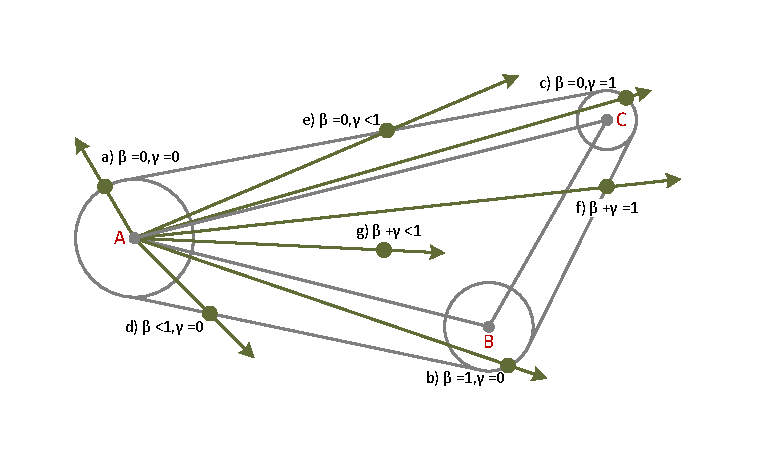
\includegraphics[width=0.6\textwidth]{./pics/text_1_remesh_common_envelope/triangle2.pdf}
\singlespacing
\captionstyle{center}\caption{Различные варианты пересечения траектории смещения узла и общей огибающей семейства сфер.}
\label{fig:text_1_remesh_common_envelope_2}
\end{figure}

Введем следующие обозначения $R_A = R(A)$, $R_{AB} = R(B) - R(A)$, $R_{AC} = R(C) - R(A)$, тогда \eqref{eqn:text_1_remesh_common_envelope_eq} можно записать в виде
\begin{equation}
	|\alpha \overline{D} - (\beta \overline{AB} + \gamma \overline{AC})|^2 = (R_A + \beta R_{AB} + \gamma R_{AC})^2,
\end{equation}

или явно как квадратное уравнение относительно переменной $\alpha$:
\begin{multline}
	|\overline{D}|^2 \alpha^2 - 2(\beta (\overline{D}, \overline{AB}) + \gamma (\overline{D}, \overline{AC})) \alpha + \\
	|\beta \overline{AB} + \gamma \overline{AC}|^2 - (R_A + \beta R_{AB} + \gamma R_{AC})^2 = 0
\end{multline}

Наибольший корень этого квадратного уравнения вычисляется следующим образом (с учетом условия $|\overline{D}| = 1$):
\begin{multline}
	\alpha(\beta, \gamma) = \beta (\overline{D}, \overline{AB}) + \gamma (\overline{D}, \overline{AC}) + \\
	\sqrt{(\beta (\overline{D}, \overline{AB}) + \gamma (\overline{D}, \overline{AC}))^2 - |\beta \overline{AB} + \gamma \overline{AC}|^2 + (R_A + \beta R_{AB} + \gamma R_{AC})^2},
\end{multline}

или
\begin{equation}
	\begin{aligned}
		& \alpha(\beta, \gamma) = k_{\beta} \beta + k_{\gamma} \gamma + \sqrt{T} \\
		& T = q_{\beta^2} \beta^2 + q_{\gamma^2} \gamma^2 + q_{\beta \gamma} \beta \gamma + q_{\beta} \beta + q_{\gamma} \gamma + q \\
		& k_{\beta} = (\overline{D}, \overline{AB}), \ k_{\gamma} = (\overline{D}, \overline{AC}) \\
		& q_{\beta^2} = (\overline{D}, \overline{AB})^2 - |\overline{AB}|^2 + R_{AB}^2, \ q_{\gamma^2} = (\overline{D}, \overline{AC})^2 - |\overline{AC}|^2 + R_{AC}^2 \\
		& q_{\beta \gamma} = 2 \left( (\overline{D}, \overline{AB}) (\overline{D}, \overline{AC}) - (\overline{AB}, \overline{AC}) + R_{AB}R_{AC} \right) \\
		& q_{\beta} = 2 R_A R_{AB}, \ q_{\gamma} = 2 R_A R_{AC}, \ q = R_A^2
	\end{aligned}
\end{equation}

Для поиска нового положения точки $A$ требуется найти максимум выражения $\alpha(\beta,\gamma)$ при условии соблюдения ограничений $\beta \ge 0$, $\gamma \ge 0$, $\beta + \gamma \le 1$.
Максимум выражения $\alpha(\beta, \gamma)$ достигается либо при условии нахождения центра сферы внутри треугольника $ABC$ , либо на одной из его сторон.
В случае нахождения центра сферы на стороне $AB$ треугольника $ABC$ выполняется условие $\gamma = 0$, и выражение для величины $\alpha$ имеет вид
\begin{equation}
	\alpha_{\gamma = 0} = k_{\beta} \beta + \sqrt{q_{\beta^2} \beta^2 + q_{\beta} \beta + q}.
\end{equation}

В случае нахождения центра сферы на стороне $AC$ треугольника $ABC$ выполняется условие $\beta = 0$, и выражение для вели-
чины $\alpha$ имеет вид
\begin{equation}
	\alpha_{\beta = 0} = k_{\gamma} \gamma + \sqrt{q_{\gamma^2} \gamma^2 + q_{\gamma} \gamma + q}.
\end{equation}

В случае нахождения центра сферы на стороне $BC$ треугольника $ABC$ выполняется условие $\beta + \gamma = 1$, и выражение для величины $\alpha$ имеет вид
\begin{multline}
	\alpha_{\beta + \gamma = 1} = (k_{\gamma} - k_{\beta}) \gamma + k_{\beta} + \\
	\sqrt{(q_{\beta^2} + q_{\gamma^2} + q_{\beta \gamma}) \gamma^2 + (-2 q_{\beta^2} + q_{\beta \gamma} - q_{\beta} + q_{\gamma}) \gamma + (q_{\beta^2} + q_{\beta} + q)}
\end{multline}

Во всех случаях нахождения центра сферы на одной из сторон треугольника задача нахождения максимального значения $\alpha(\beta, \gamma)$ при заданных ограничениях сводится к задаче поиска максимального значения функции вида $\alpha(x) = k_x x + k + \sqrt{q_{x^2} x^2 + q_x x + q}$ (с учетом этих ограничений), что является аналогом задачи поиска пересечения прямой и окрестностью отрезка, описанной в разделе \ref{sec:text_1_geo_prim_line_eps_intersect}, (точкой максимума является либо точка локального экстремума, либо точка, находящаяся на границе области определения функции).

Отдельно рассмотрим вариант, когда центр искомой сферы находится внутри треугольника.
В этом случае точка пересечения траектории $\overline{P}(\alpha) = \overline{A} + \alpha \overline{D}$ находится на общей касательной плоскости к сферам $Sphere(0,0)$, $Sphere(1,0)$, $Sphere(0,1)$ (плоскость $A'B'C'$, см. рис.~\ref{fig:text_1_remesh_common_envelope_3}).

\begin{figure}[ht]
\centering
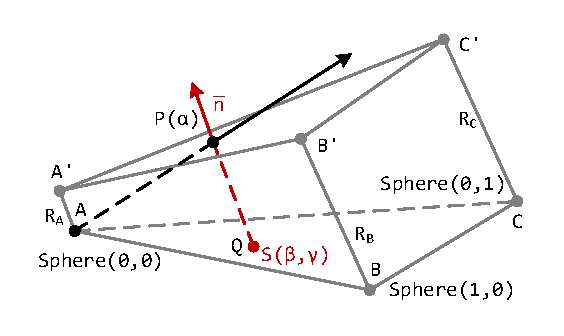
\includegraphics[width=0.7\textwidth]{./pics/text_1_remesh_common_envelope/case1.pdf}
\singlespacing
\captionstyle{center}\caption{Случай нахождения пересечения траектории движения точки с границе окрестности ячейки, если центр сферы лежит внутри треугольника.}
\label{fig:text_1_remesh_common_envelope_3}
\end{figure}

Центр искомой сферы находится в точке пересечения плоскости $ABC$ и прямой, проходящей через точку $\overline{P}(\alpha)$ и направленной вдоль нормали к плоскости $A'B'C'$ .
Если вектор единичной нормали плоскости $A'B'C'$ обозначить через $\overline{n}$, то взаимосвязь точек плоскостей $ABC$ и $A'B'C'$ можно выразить следующим образом:
\begin{equation}
	\begin{aligned}
		\overline{A}' = \overline{A} + \overline{n}R_A \\
		\overline{B}' = \overline{B} + \overline{n}R_B \\
		\overline{C}' = \overline{C} + \overline{n}R_C
	\end{aligned}
\end{equation}

Для нахождения вектора $\overline{n}$ используем тот факт, что результат векторного произведения $\overline{A'B'} \times \overline{A'C'}$ коллинеарен вектору $\overline{n}$.
Запишем это в явном виде
\begin{equation}
	(\overline{AB} + \overline{n} R_{AB}) \times (\overline{AC} + \overline{n} R_{AC}) = t \overline{n}
\end{equation}

\begin{equation}
	\overline{AB} \times \overline{AC} + R_AB(\overline{n} \times \overline{AC}) - R_{AC}(\overline{n} \times \overline{AB}) = t \overline{n}
\end{equation}

\begin{equation}\label{eqn:text_1_remesh_common_envelope_matr}
	t
	\begin{pmatrix}
		n_x \\
		n_y \\
		n_z
	\end{pmatrix}
	+ R_{AC}
	\begin{pmatrix}
		n_y AB_z - n_z AB_y \\
		n_z AB_x - n_x AB_z \\
		n_x AB_y - n_y AB_x
	\end{pmatrix}
	- R_{AB}
	\begin{pmatrix}
		n_y AC_z - n_z AC_y \\
		n_z AC_x - n_x AC_z \\
		n_x AC_y - n_y AC_x
	\end{pmatrix}
	= \overline{AB} \times \overline{AC}
\end{equation}

Соотношение \eqref{eqn:text_1_remesh_common_envelope_matr} может выполняться как при $t > 0$, так и при $t < 0$, что соответствует существованию двух общих касательных плоскостей к трем сферам.
Перепишем приведенное соотношение в виде системы линейных уравнений относительно составляющих нормали при произвольном значении параметра $t$.
\begin{multline}\label{eqn:text_1_remesh_common_envelope_matr2}
	\begin{pmatrix}
		t                         & R_{AC} AB_z - R_{AB} AC_z & R_{AB} AC_y - R_{AC} AB_y \\
		R_{AB} AC_z - R_{AC} AB_z & t                         & R_{AC} AB_x - R_{AB} AC_x \\
		R_{AC} AB_y - R_{AB} AC_y & R_{AB} AC_x - R_{AC} AB_x & t
	\end{pmatrix}
	\begin{pmatrix}
		n_x \\
		n_y \\
		n_z
	\end{pmatrix} \\
	= \overline{AB} \times \overline{AC}
\end{multline}

Из системы уравнений \eqref{eqn:text_1_remesh_common_envelope_matr2} находятся два возможных направления нормали к общей касательной плоскости для сфер $Sphere(0,0)$, $Sphere(1,0)$, $Sphere(0,1)$.
Для каждого направления нормали находится плоскость $A'B'C'$ и точка $\overline{P}(\alpha) = \overline{A} + \alpha \overline{D}$ на ней (и сам искомый параметр $\alpha$).
Эту точку можно учитывать в общем наборе решений только в том случае, если ей соответствует сфера $Sphere(\beta, \gamma)$, параметры которой удовлетворяют условиям $\beta \ge 0$, $\gamma \ge 0$, $\beta + \gamma \le 1$.
Параметры $\beta$, и $\gamma$ можно определить путем поиска точки пересечения прямой $\overline{P}(\alpha) - x \overline{n}, x \in \mathbb{R}$ и плоскости $ABC$.

Таким образом, найдя решения всех потенциально возможных частных случаев, представленных на рис.~\ref{fig:text_1_remesh_common_envelope_2}, находим множество решений $\alpha$ , из которых для определения актуального нового положения точки $A'$ необходимо выбрать максимальное.
На этом определение смещения узлов расчетной сетки завершено.

Изложенный выше алгоритм касается определения смещения узла с учетом только одной инцидентной ячейки.
При рассмотрении отдельного узла расчетной сетки требуется вычислить смещение этого узла относительно каждой инцидентной ячейки и выбрать среди этих смещений максимальное (см. рис.~\ref{fig:text_1_remesh_common_envelope_4}).
На рис.~\ref{fig:text_1_remesh_common_envelope_4} представлена двумерная иллюстрация действия алгоритма на примере затягивания небольшой впадины.
Видно, что результирующая поверхность получилась более гладкой, хоть некоторые ячейки и стянулись в более мелкие.
Для повышения качества сетки можно выполнить удаление слишком мелких ячеек.

\begin{figure}[ht]
\centering
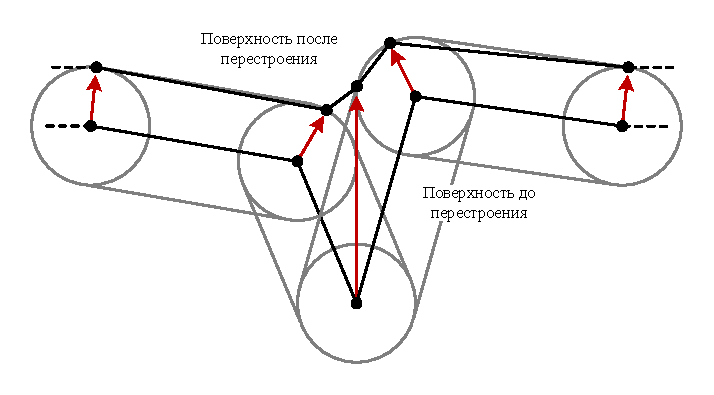
\includegraphics[width=0.6\textwidth]{./pics/text_1_remesh_common_envelope/out_from_cave.pdf}
\singlespacing
\captionstyle{center}\caption{Схема стягивания впадины после одного шага алгоритма перестроения поверхности с использованием окрестности ячейки.}
\label{fig:text_1_remesh_common_envelope_4}
\end{figure}

\begin{figure}[ht]
\centering
\begin{tabular}{ll}
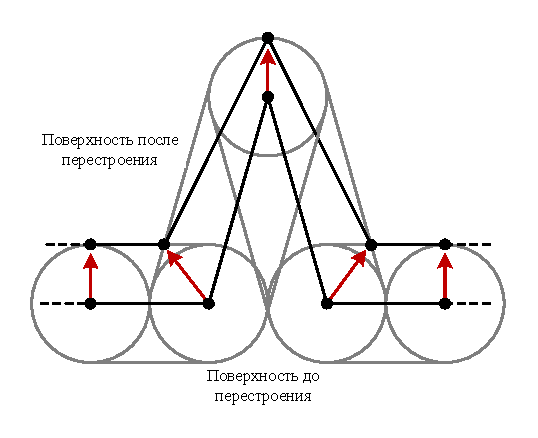
\includegraphics[width=0.45\textwidth]{./pics/text_1_remesh_common_envelope/peak1.pdf}
&
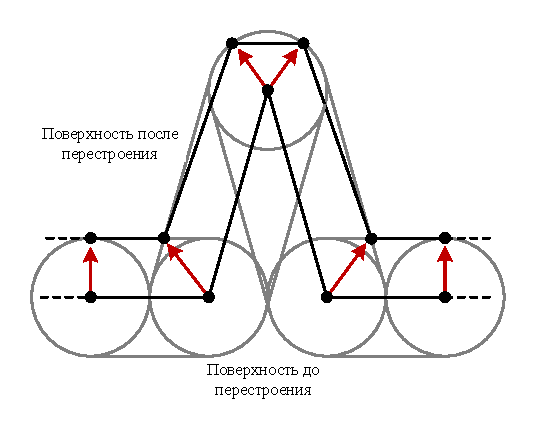
\includegraphics[width=0.45\textwidth]{./pics/text_1_remesh_common_envelope/peak2.pdf}
\end{tabular}
\singlespacing
\captionstyle{center}\caption{Сглаживание острых выпуклых пиков поверхности в результате работы алгоритма.}
\label{fig:text_1_remesh3_common_envelope_peak}
\end{figure}

Другим интересным случаям является результат работы алгоритма на участках сетки с острыми выпуклыми пиками (рис.~\ref{fig:text_1_remesh3_common_envelope_peak}).
Из данного рисунка видно, что в результате работы алгоритма острый угол сглаживается, и при продолжении наращивания льда в несколько итераций сглаживание продолжится (рис.~\ref{fig:text_1_remesh3_common_envelope_peak}, слева).

Следует отметить, что на таких острых пиках несколько снижена точность по объему льда.
Эту точность можно повысить путем добавления новых узлов расчетной сетки и корректировки направлений смещения получившихся вершин (рис.~\ref{fig:text_1_remesh3_common_envelope_peak}, справа).

В результате реализации описанного алгоритма удалось получить программный модуль, способный обрабатывать поверхностные расчетные сетки произвольной сложности и содержащие дефекты.
Также алгоритм не содержит итерационных процедур сглаживания и является линейным по количеству узлов в расчетной сетке.

\begin{figure}[ht]
\centering
\begin{tabular}{ll}
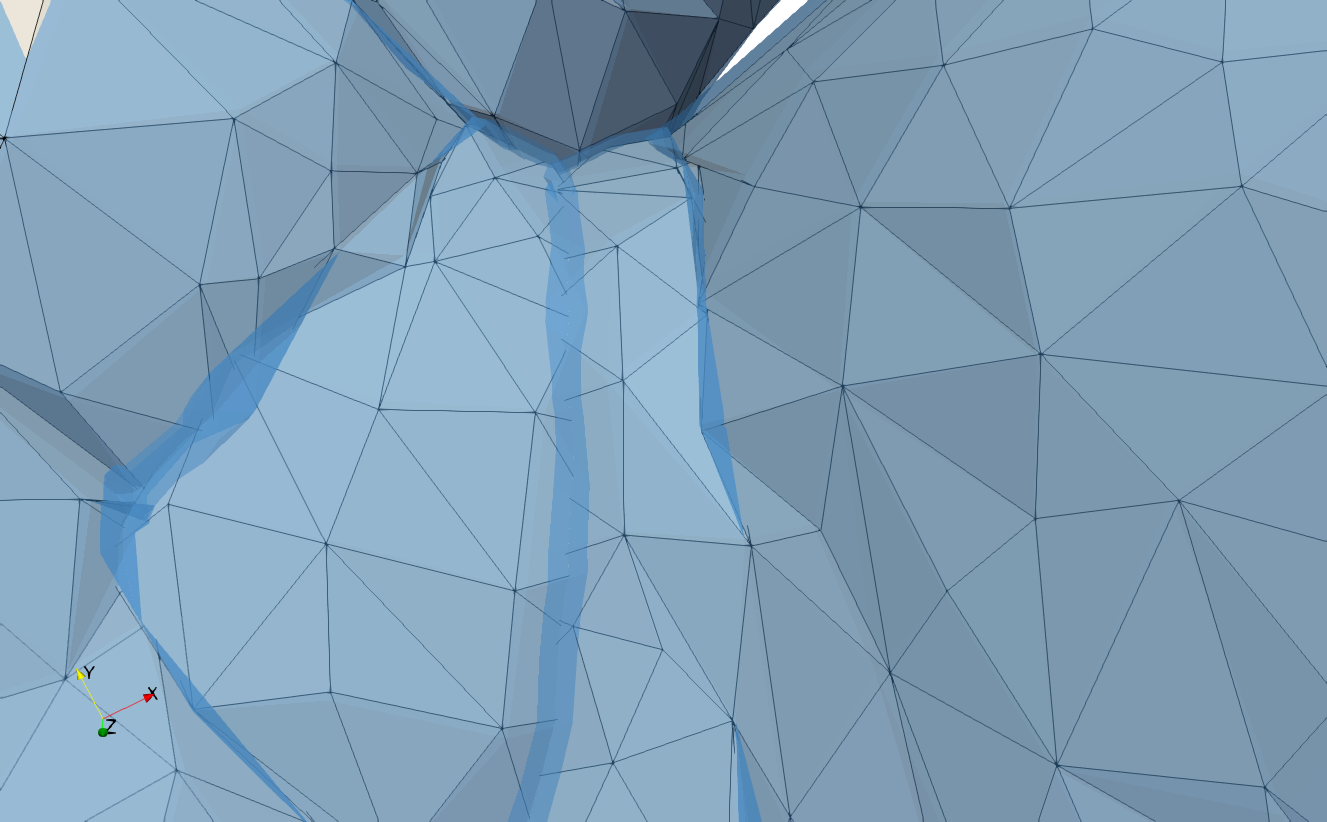
\includegraphics[width=0.45\textwidth]{./pics/text_1_remesh_common_envelope/pic_envelope_cave.png}
&
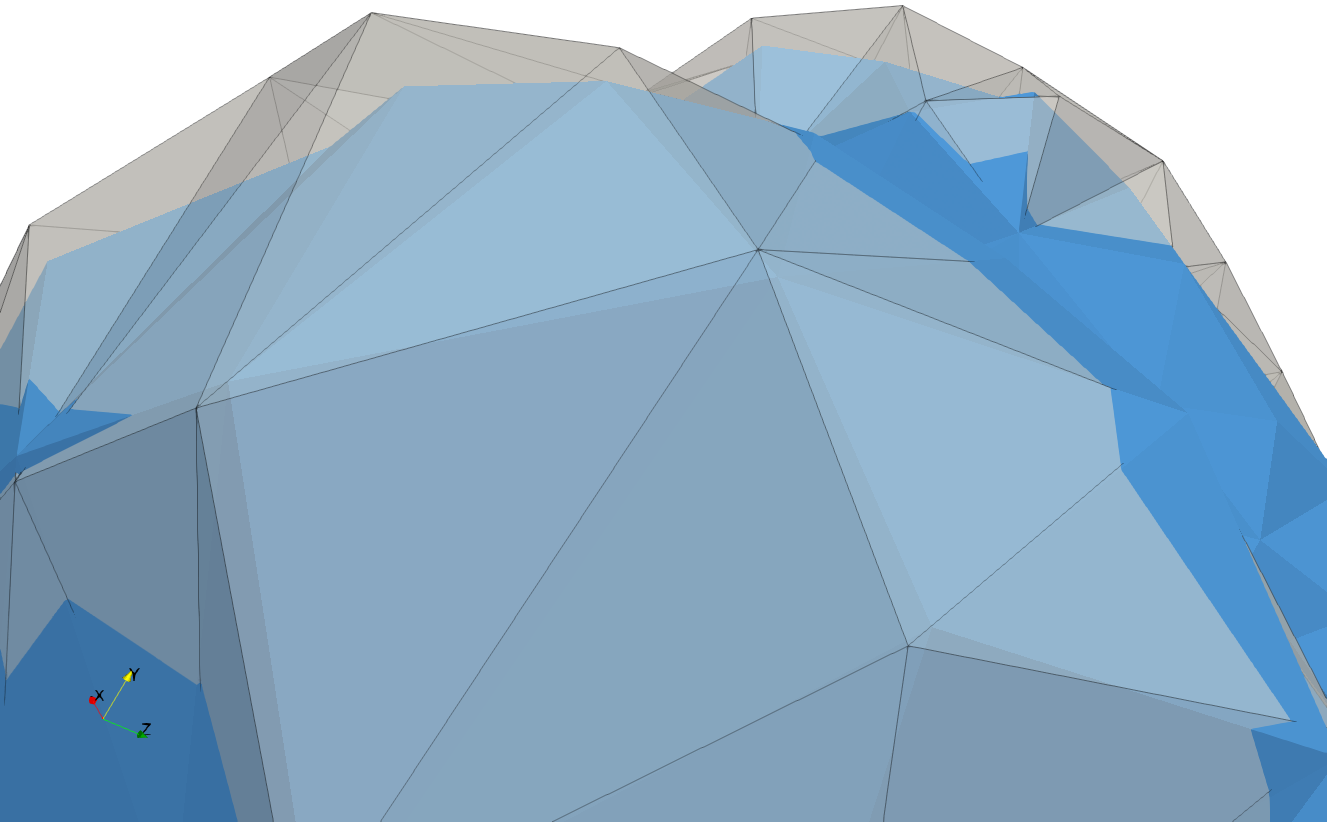
\includegraphics[width=0.45\textwidth]{./pics/text_1_remesh_common_envelope/pic_envelope_peak.png}
\end{tabular}
\singlespacing
\captionstyle{center}\caption{Результат работы алгоритма перестроения сетки на тестовой сетке.}
\label{fig:text_1_remesh3_common_envelope_bunny}
\end{figure}

На рис.~\ref{fig:text_1_remesh3_common_envelope_bunny} продемонстрирована работа алгоритма перестроения поверности с использованием окрестности ячейки на тестовой расчетной сетке.
На рис.~\ref{fig:text_1_remesh3_common_envelope_bunny} слева показано сглаживания мелких впадин по сравнению с перестроением с помощью метода призм.
На рис.~\ref{fig:text_1_remesh3_common_envelope_bunny} справа показан эффект сглаживания острых пиков по сравнению с перестроением с помощью метода пирамид\label{term:method_remesh_pyramid2}.

\begin{figure}[ht]
\centering
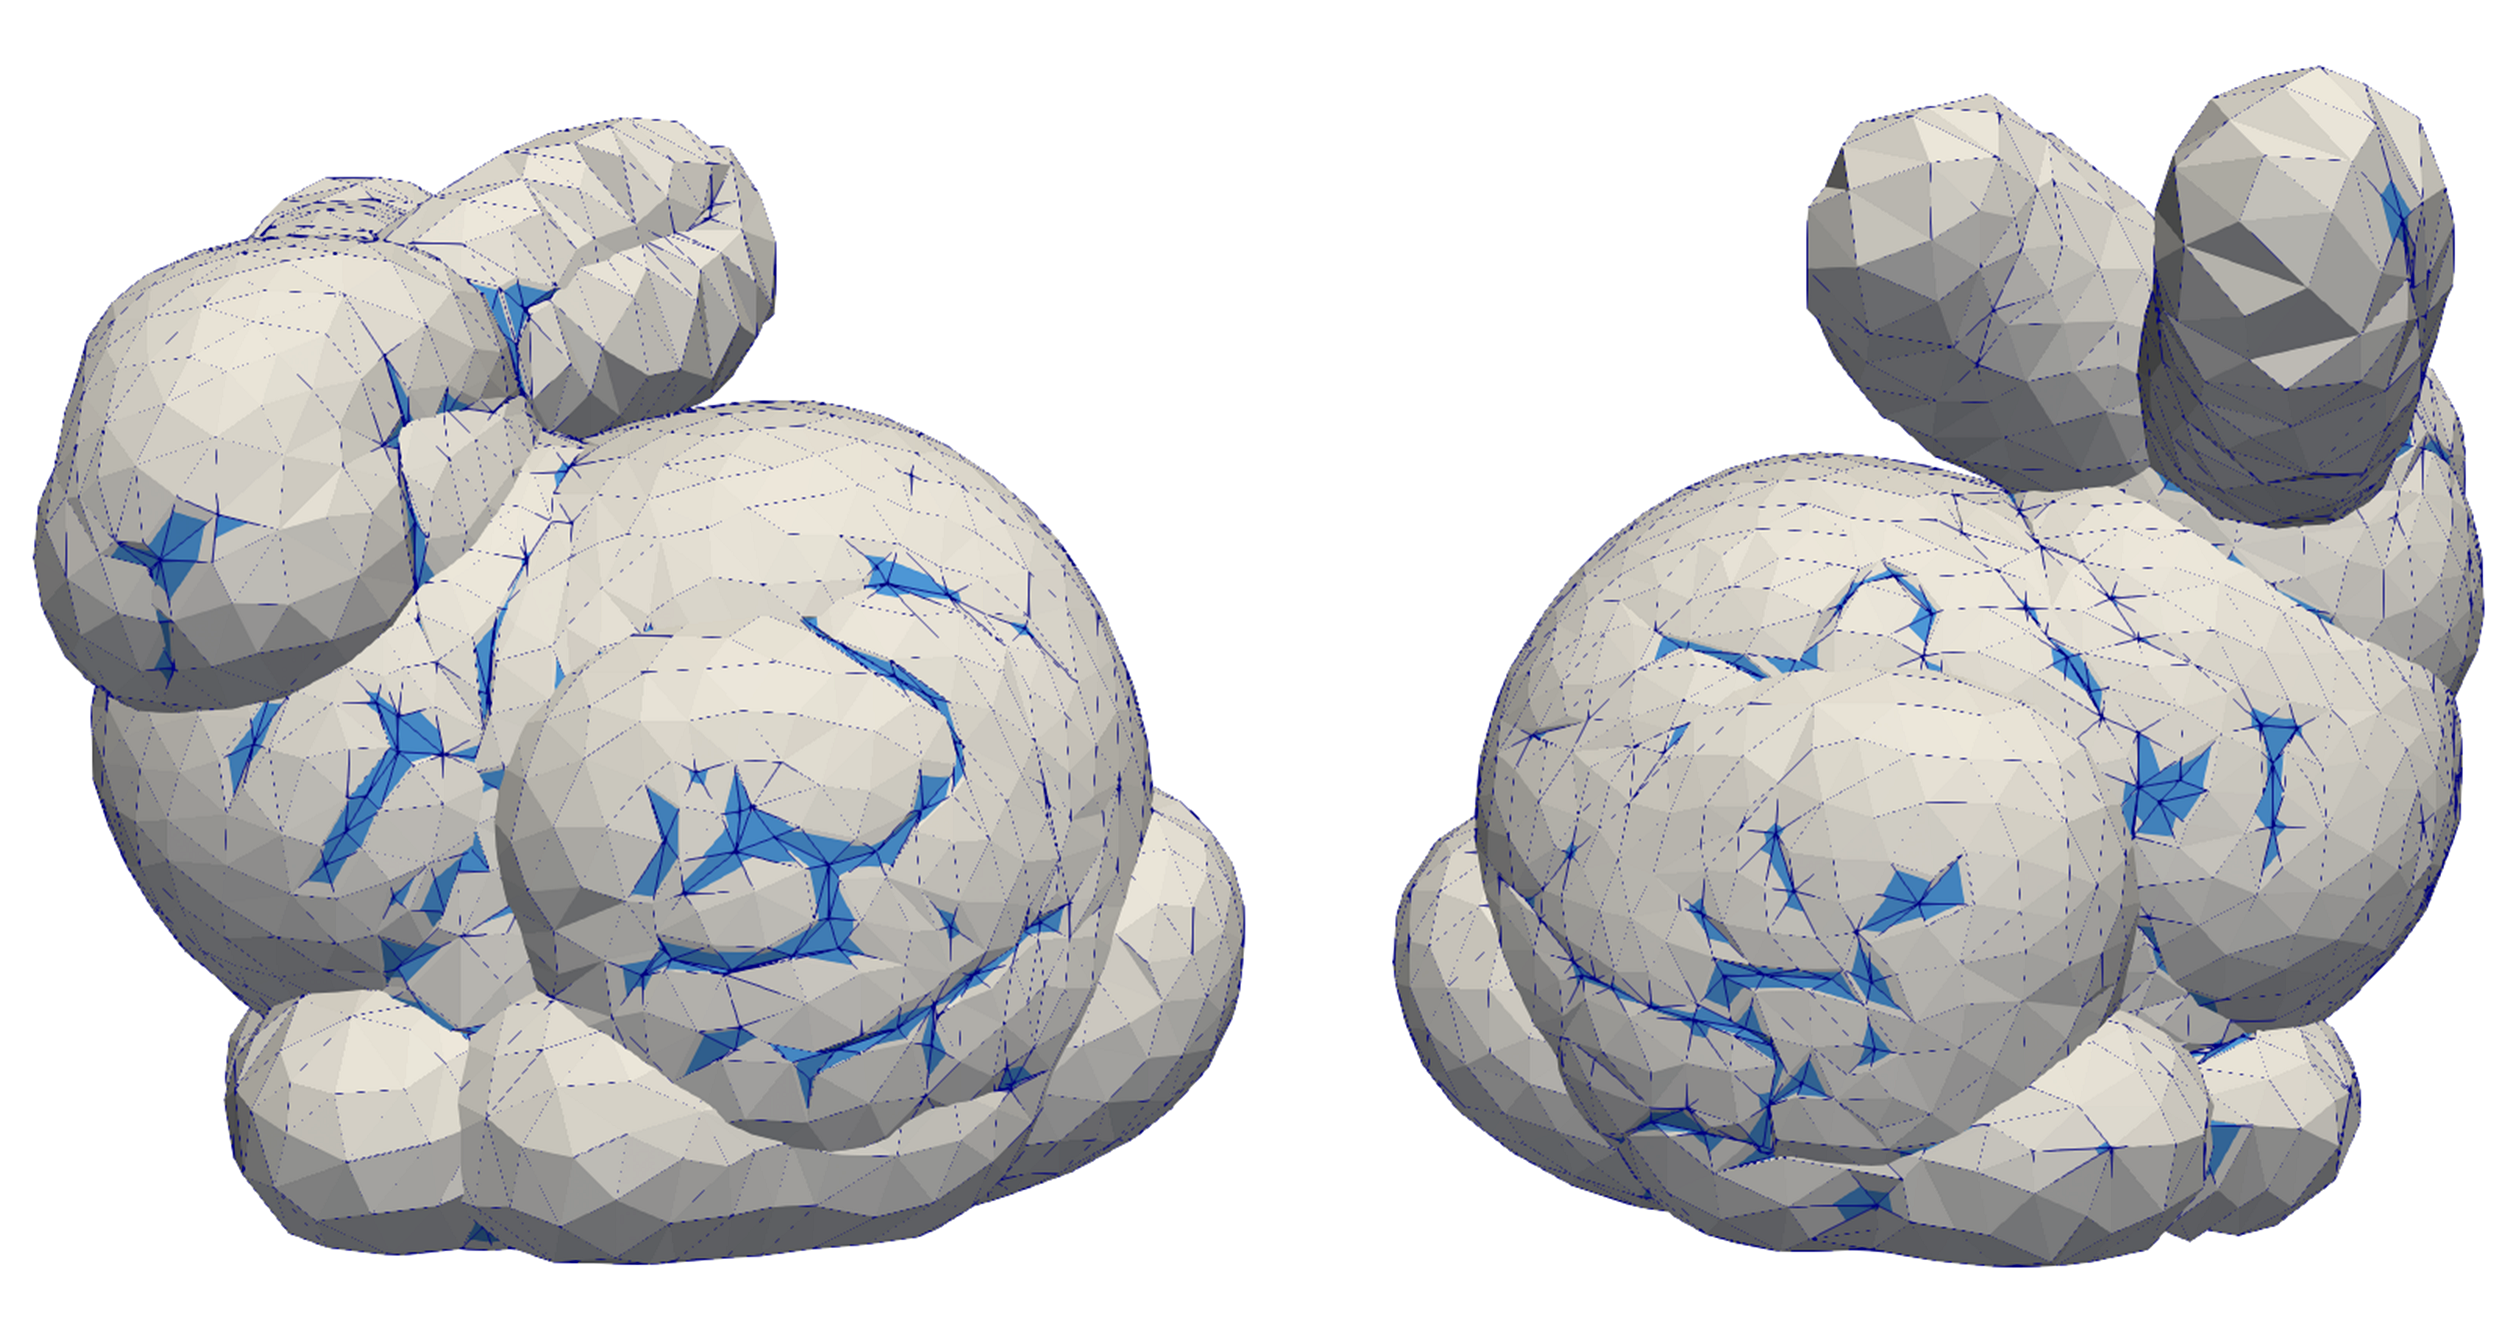
\includegraphics[width=0.9\textwidth]{./pics/text_1_remesh_common_envelope/bunny.png}
\singlespacing
\captionstyle{center}\caption{Демонстрация сглаживания мелких впадин на тестовой сетке.}
\label{fig:text_1_remesh3_common_envelope_bunny2}
\end{figure}

На рис.~\ref{fig:text_1_remesh3_common_envelope_bunny2} продемонстрирована работа алгоритма на тестовой расчетной сетке.
На этом рисунке видно затягивание мелких впадин и складок (отмечено синим цветом).